\documentclass[a4paper, 11pt]{article}
%\documentclass[10pt,a4paper,twocolumn]{article}
\usepackage{amssymb,amsmath}
\usepackage{graphicx}
%\usepackage{times}
%\usepackage{float}
\usepackage{algorithmic}

\title{Distributed Peer-to-peer File System}  
\author{Darius Scerbavicius} 
\date{4th April 2013}

\begin{document}

\maketitle

\begin{abstract}
%TODO: rewrite this but you get the idea
Although the popularity of services similar to DropBox and Google Drive proves that 
users find such cloud storage file hosting services useful,
currently no decentralised and distributed file system exists that could provide
a service of similar quality but without dependence on any single vendor.
%a file system requires solving lots of problems, such as file persistence, security, 
%good behaviour on network failure etc. Testing such an implementation is also not easy,
%as simulating real network behaviour is hard. 
This project attempts to implement such a system,
and to provide a comparison to other systems with similar goals, by using common
file system benchmarks. 

A prototype of the file system backend has been implemented, and a testing environment
using LXC has been setup and evaluated to determine its suitability for testing the 
file system service.

\end{abstract}

\section{Introduction}

A number of companies are providing a remote synchronized directory service, with the most famous examples being Dropbox \cite{dropbox} and Google Drive \cite{gdrive}. These services are not deployed in a peer-to-peer manner -- the user's files are stored on the servers of the company which provides the services. This means, that if the company ever goes out of business, decides to stop offering the service, or simply changes the terms of the service to ones that the user disagrees with, the user will no longer be able to use the service. 
Furthermore, the proposed project has the potential to offer much more free space to its users than any of the currently available centralised services.

During the last 15 years, a lot of promising technology has been developed that can eliminate the providing vendors while offering the same high quality service. 
Systems based on a Distributed Hash Table (DHT) have allowed lookup services to be implemented in a completely decentralised network, allowing any participating nodes to efficiently retrieve data. Implementations of DHTs are being successfully used in various peer-to-peer Internet services, such as BitTorrent and Coral Content Distribution Network \cite{coral}.

Such technology is just as well applicable to distributed file systems. Attempts to implement such systems have been made, with the most prominent names being   CFS \cite{cfs}, Pastis \cite{pastis}, OceanStore \cite{oceanstore}, Ivy \cite{ivy}, Infinit \cite{towards}. So far no implementations are being used outside the research community by the wider public, and no large-scale high quality open source projects capable of offering such a service have been established.

The purpose of this MInf dissertation is to build a Distributed Peer-to-peer File System, capable of performing similar function to the proprietary services such as DropBox \cite{dropbox}, but without depending on any specific vendor, so that the contents of the person's private folder are encrypted and then distributed among other users of the system. 
%
%The project consists of developing a back-end based on a peer-to-peer distributed hash table algorithm, and a front-end, which would allow users to place and retrieve files from the file system.
%
%\section{Problems}

%A distributed file system capable of providing a high quality service must solve a very large set 
%of problems:

%TODO: describe some background for each of them?
%\begin{itemize}
%\item Security
%\item Scalability
%\item Replication
%\item Version control
%\item Access control
%\item Evaluating such a system
%\end{itemize}

% Project & Goals
% Develop a P2P distributed file system 
%
% DHT - Chord
%
% Approach
% Unaddressed problems
% File persistence (has this been addressed in any way?)
% Security (encrypted file contents)
% Reading files larger than there currently is space available
%
% Cannot use planet lab, emu lab, because university does not give me access
% proposing a testing system, that allows running multiple nodes (cite paper about bit torrent and lxc)
% results of running simple chord in such a networked system 
%
% Workplan (detailed, exact milestones)

\section{Project Overview}

The following section will present a complete view of the project, using a bottom-up approach, starting from the lowest protocol level and ending with the design of the frontend. 

\subsection{Key-Based Routing}
%Ivy�s lack of support for automatically adding new users
%to a view is intentional.
%
%pastis

The lowest level of the distributed file system is built on a key-based routing protocol, Chord. The purpose of this level is, given a key and a message, to route the message to the node with an identifier closest to the key. In our case, the key is the SHA-1 hash of the file path, and the identifier is the SHA-1 hash of the IP address of the node. The distance between the node's identifier and the key of the message is determined by taking the difference between them. %(talk about chord's routing algorithm like in CFS paper)

Each node in the network is connected to a set of other nodes (its neighbours) by a number of links (the routing table).

Chord can be imagined as a network of nodes connected in a ring, where each node knows its successor (the next node in clockwise direction) and its predecessor (next node in counter-clockwise direction). Consistent hashing is used to assign keys to nodes, which balances the load on the network. The value of a key-value pair is assigned to the first node that has an identifier equal to the key, or an identifier that follows the key. 

Nodes maintain a routing table that accelerates lookups. In a system of $N$ nodes, a lookup can be resolved using $O(log N)$ messages to other nodes, suggesting high performance, suitable for a peer-to-peer file system \cite{chord}.


% what are the main reasons to use chord instead of other KBRs?

%(how does chord scale?)

\subsection{Distributed Hash Table}

On top of this lowest level, sits the DHT (distributed hash table). Like a hash table, a DHT provides a mapping from keys to values. It allows inserting a value with a certain key, and allows the value to be retrieved, by providing the key that was used to insert it. The DHT operates on a network of nodes, and uses the key-based routing protocol to determine the sought node. The DHT used for this distributed filesystem will be based on CFS DHash.
% again, why CFS DHash?

In order to be suitable for usage in a distributed file system, The DHT must provide an interface supporting the following operations:

\begin{itemize}
\item insert(key, value)

The DHT will use Chord to determine which node the key value pair should be stored on. To ensure file system persistence, replicas of the value will be stored on k number of nodes coming after the successor of the picked node. It should be noted that the number k has not yet been determined. 

\item retrieve(key)

Again, the DHT will use Chord to determine the node carrying the value given by the key. As k number of nodes following that node store a replica of the requested value, the latency to each of them will be measured, and the fastest node will be picked for downloading.

\item delete(key)

Deletion will be implemented simply by deleting the file path from the user's file record (which will be discussed further). To an extent, this also guards against malicious injections of large amounts of data \cite{cfs}, as such data will be gradually deleted.
\end{itemize}
TODO: address caching

As the file system may be deployed on storage drives of varying size, including ones that provide less space than some of the files stored on the world-wide file system, the DHT will divide the files into smaller blocks suitable for storage. 

%TODO: describe how CFS does this

\section{Security}

The prototype implementation will not have a sophisticated access control system. A simple mechanism based on public key encryption and digital signatures will be provided instead. 

Each user of the file system must have generated a private key, which is used to encrypt all files, and a public key.

% TODO: signatures

\section{File System Structure}

The list of files stored on the file system by the user, will be governed by an index. As in CFS, this index will be stored under the user's public key. The current plan is to maintain the index as a plain text file, although this is obviously inadequate for file systems containing large numbers of files. A more sophisticated approach, involving a database, will be presented later. 

Whenever a user creates a new file, a record of the file will be added to the index, and likewise the file's record will be deleted when the user deletes that particular file.

To connect to the system, a user must first obtain an IP address of a node already in the system. The node would 

The file system will be implemented in a modular way. %TODO: what do you mean

\section{Evaluation}

The University of Edinburgh does not have access to PlanetLab
The evaluation testbed and methods were chosen after a careful assessment of a number of different procedures, under the criteria that:
\begin{enumerate}
\item no significant differences would be required between the implementation used in the simulation, and the implementation used in the real world;
\item the simulation would be capable of running a large amount of nodes ($>$ 2000).
\item there would be a good basis to believe that the obtained results are applicable to the real world;
\end{enumerate}

\subsection{ns-3}
The first method considered, was to target ns-3 for the test bed environment, as it has previously been used for this purpose when testing the Infinit file system. This method was attempted, but its main drawback is that the implementation used in simulation would differ too much from the implementation targeting the real world.

% TODO: explain how ns3 could be used to do this

\subsection{LXC Containers}

The file system will be tested using a local emulation testbed. The testbed uses Linux Containers (LXC), a high-performance operating system level virtualization solution, that allows sharing the resources of the host machine among many isolated instances. LXC containers use the Linux kernel cgroups feature to segregate processes, isolating them from other processes, and providing them with their own network space. FUSE-based file systems can be mounted on LXC containers, but the containers can also share certain directories with the host machine.

Such a testbed has previously been used for analyzing the performance of a P2P swarm \cite{p2plxc} using the hrktorrent BitTorrent client, and bttrack BitTorrent tracker. Each peer was running in its own container, on top of the hardware node, sharing parts of the system with the host, and very little decrease in download speed was noted when the number of peers was gradually increased from 20 to 100. This is surprising, as a very low-end machine was used for executing the tests (Intel(R) Core(TM)2 Duo CPU T7500 @ 2.20GHz, 1.5 GB of RAM), indicating that the LXC containers have a very low overhead, and running a large amount of nodes is possible.

Nevertheless, even a powerful machine may not be able to handle a very large number of nodes running the P2P filesystem. As LXC containers have their own network device configuration, it is possible to expose them to the wider network. The plan is then to have a number of machines running LXC containers, each contributing a different amount of peers to the filesystem network, depending on the machine's resources.


% topologies?

\section{Current Progress}

Most work done so far has been on preparing a suitable testing environment for testing the filesystem.

The first attempt consisted of implementing a subset of Chord (without support for the routing tables), and a simplistic DHT layer on top of it, using ns-3. As ns-3 has support for Python bindings, it seemed as the language of choice, but after taking further steps, the Python binding documentation turned out to be very inadequate, and some important parts of the API, such as callbacks, turned out not to be properly supported in Python.  

This instigated a switch to using C++ for development, and using the proper C++ API of ns-3. However, as the development of the Chord protocol proceeded, it became clear that, although the parts of the ns-3 API relevant to this project are similar to the Unix sockets API (which is in fact one of the main selling points of ns-3), there is still too much of a difference between them.

However although ns-3 API has its own API, it was clear that such an implementation would be too different from the one targeting the real world.

\begin{figure}
\begin{center}
  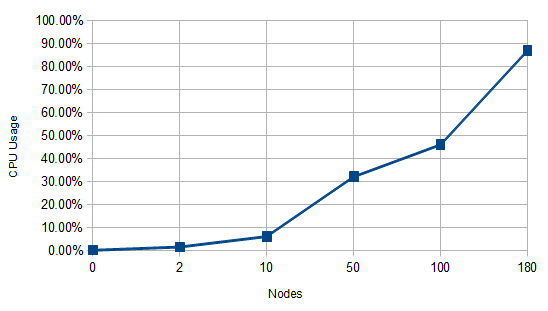
\includegraphics[width=11cm]{cpu_nodes.png}
\end{center}
\caption{Control flow states}
\label{flow}
\end{figure}  


\section{Future Plans}

The current goal of the project is to get the file system to a state where the ANDREW benchmark can be executed on it. At that point it will be possible to compare the speed of the file system to NFS, and this will make it clearer as to how well it scales when nodes are added/removed, and what its most significant short-comings are in regards to other similar file systems.

With these taken into account, the modularity of the system will allow 

\section{Work Plan}


%SHIT LEFT TO COVER:
%quorum crap?
%security?
%malicious nodes?
%overwriting files?
%
%introduction
%workplan
%
%main problem with infinit: evaluation does not deal with churn

% As such, each user maintains a file list, of all files in
%the system that belong to the user.
%The current approach is to disregard all access control, and solve the issue later.
%
%
%% could copying be implemented in a clever way? how do other file systems do it?
%\section{Purpose}
%
%The project will strive for:
%\begin{enumerate}
%\item simplicity, so that potential open source contributors find the project easy to grasp, thus enabling them to submit contributions;
%\item efficiency, since users will only consider the file system useful if it offers good performance.
%\end{enumerate}
%
%\section{Background}
%
%
%A list of decentralised peer-to-peer file systems and their drawbacks follows:
%
%\begin{description}

%\section{Methods}
%
%And essentially no fully decentralised file system has been adopted by the wider public. 
%To build such a file system, a back-end and a front-end will be designed.
%
%The base of the back-end of such a system is a DHT (distributed hash table), capable of executing three commands among all nodes:
%The novelty of the system lies in being able to keep more files in the cloud, than there currently is space available on your physical hard drive. 
%
%This will be done by maintaining a list of the most frequently or recently used files that will be cached in the system, while leaving the rest of the space (that was allocated to the file system by the user) for keeping reconds of other people's files that they stored in the cloud.
%
%This should be possible, as the encouraged behaviour for a user of such a file system, is to allocate a large amount of hard drive space to it, but it is likely that the user will only use a small amount of that space for his or her own files (which are then going to be uploaded to this 'cloud' anyway).
%
%Describe how quorums are stored in the system,
%
%How we go from FUSE to executing all of the above (check FUSE API)
%
%Protocol needs to be scalable (as there might be a lot of nodes connected, how to address that?), also needs to support churn, as network nodes will move in and out of the network.
%
%Steps to editing a file:
%\begin{enumerate}
%\item user access a file on his/her file system
%\item retrieve(key) is called
%\item user edit and saves the file
%\item insert(key, value)
%\item update is propagated according to quorum rules
%\end{enumerate}
%
%Also need to address: security, persistence (how exactly am I adding sth new to the area)
%\begin{itemize}
%\item The back-end will be based on a DHT (Distributed Hash Table). 
%\item The front-end of the file system will be based on FUSE (Filesystem in Userspace) \cite{fuse}.
%\end{itemize}
%The implementation will target a real world workload. The ns-3 \cite{ns3} simulator will be used to test the implementation.
%
%\section{Current Progress}
%
%Work done so far consisted of a prototype implementation of the Chord protocol on top of the Python Twisted networking library, and a setting up of a testing infrastructure, capable of determining whether 
%\subsection{Network}
%\subsection{Replication}
%To enable reliable file storage, the peer-to-peer network must have a system of file replication. The most basic implementation is to store the exact same replica of the file at a fixed number of successor nodes. This is in fact the suggested method for higher level applications by Chord authors \cite{chord}.
%
%In the case that this is deemed inadequate during the development process, a more complicated scheme, such as Dynamic Replication could be implemented instead \cite{dhash}.
%
%\subsection{Versioning}
%Due to the way replication works, not all copies of the file currently in the network are going to be up-to-date. To ensure that the user always receives the most recent copy, when performing a lookup, a weighted voting scheme is going to be introduced. The replicas will be assigned a version number, and each replica of a file will be assigned a certain number of votes. Whenever the file is accessed, or written to, a certain number of $r$ votes to read a file, and a certain number of $w$ votes to write a file will be collected, such that $r + w$ is more than the total number of votes assigned to file. This guarantees that any lookup will always retrieve the most recent version of the file \cite{versioning}.
%
%\subsection{Cryptography}
%
%Unlike other Peer-to-peer systems such as Freenet, the emphasis of this project is not anonymity, but instead simplicity and efficiency. Only a minimal security mechanism will be provided, where the owner's files will be encrypted using a symmetric-key algorithm, with a possible candidate being Twofish (which is being widely used in a lot of products \cite{twofishprod}).
%This will not provide complete anonymity but will prevent unauthorised access to the user's files, as long as the key is kept safe.
%
%\subsection{Access Control}
%
%Providing an access control system is not in the scope of this project, and the task of implementing such a system is left to a higher-level application. However, an API will be provided in order to make this possible. 
%
%Since the contents of the files stored on the file system will be encrypted with the owner's key, this will to an extent prevent unauthorised access to users' resources.
%
%\subsection{Front-end}
%
%The front-end of the file system will be based on FUSE, which allows implementing a file system as a user space program \cite{fuse}. This would bypass the operating system kernel, leading to greater portability, as FUSE is available for Linux, FreeBSD, NetBSD, OpenSolaris and Mac OS X. FUSE is suitable for long-term projects, as it is well-maintained, and is an official component of the Linux kernel.
%
%\section{Evaluation}
%
%As was mentioned, the implementation targets a real-world setup. However, due to limited resources, the simulator ns-3 \cite{ns3} will be used for specific test cases. This will allow for performing simulated experiments on systems involving a large number of nodes in order to determine how well the system scales, as well as performing real-world experiments with the intent of comparing performance to other well-established file systems.
%
%\begin{itemize}
%\item Well-established and commonly used benchmarks in file system evaluation are the Andrew benchmark \cite{andrew}, and the Linux kernel build \cite{kernelb}. The results obtained from running these benchmarks would be compared to results presented in other file system papers.
%
%\item As it is common to compare the performance of peer-to-peer file systems to the performance of NFS \cite{oceanstore} \cite{ivy} \cite{pastis}, a number of real world experiments would be structured upon simple operations executed on NFS, and a comparison would be produced.
%\end{itemize}
%
%\section{Outputs}
%
%A prototype of the system described will be made available as an open source project under the GPL \cite{gpl} license. The implementation will consist of a front-end and a back-end, providing full usage capabilities on any Linux-based operating system, as well as Mac OS X. Windows will not be supported, due to the lack of a mature port of FUSE. 
%
%The project will be published on a GitHub \cite{github} repository, and open to contributions from the open source community.
%
%\section{Workplan}
%
%The workplan timetable is given below (removed).
%
%As the project progresses, it is likely that changes will be made to the timetable.

\bibliographystyle{IEEEtran}
\begin{thebibliography}{10}
\bibitem{dropbox}
Dropbox. http://www.dropbox.com/
\bibitem{gdrive}
Google Drive. http://drive.google.com/start/
\bibitem{coral}
M. J. Freedman, E. Freudenthal, D. Mazieres.
Democratizing content publication with Coral.
In NSDI, Mar. 2004.
\bibitem{ns3}
ns-3. Discrete-event network simulator. http://www.nsnam.org/
\bibitem{chord} 
I. Stoica, R. Morris, D. Karger, M. F. Kaashoek, and
H. Balakrishnan. Chord: A scalable peer-to-peer lookup
service for internet applications. In Proceedings of the 2001
Conference on Applications, Technologies, Architectures,
and Protocols for Computer Communications, pages
149–160. ACM Press, 2001.
\bibitem{fuse}
FUSE: Filesystem in Userspace. http://fuse.sourceforge.net/ 
\bibitem{cfs}
F. Dabek, M. F. Kaashoek, D. Karger, R. Morris, and I. Stoica. Wide-area
cooperative storage with CFS. In SOSP, Oct. 2001.
\bibitem{oceanstore}
J. Kubiatowicz, D. Bindel, Y. Chen, S. Czerwinski, P. Eaton, D. Geels, R. Gummadi, S. Rhea,
H. Weatherspoon, W. Weimer, C. Wells, and B. Zhao. Oceanstore: An architecture for globalscale persistent store. In Proc. ASPLOS’2000, Cambridge, MA, November 2000.
\bibitem{ivy}
A. Muthitacharoen, R. Morris, T. Gil, and B. Chen. 
Ivy: A read/write peer-to-peer file system. 
In Proc. of OSDI, 2002.
\bibitem{towards}
J. Quintard. Towards a worldwide storage infrastructure.
PhD thesis, University of Cambridge, September 2010.
\bibitem{dhash}
M. Leslie.
Reliable Data Storage in Distributed Hash Tables. Oxford University. 2005.
\bibitem{versioning}
D. K. Gifford. Weighted Voting for Replicated 
Data. In Proceedings of the Seventh ACM 
Symposium on Operating Systems Principles, 
pages 159-159, December 1979
\bibitem{twofishprod}
Bruce Schneier. Products that use Twofish. http://www.schneier.com/twofish-products.html
\bibitem{andrew}
J. H. Howard. An Overview of the Andrew File System.
In Proceedings of the Winter USENIX Technical Confer-
ence, February 1988.
\bibitem{kernelb}
A. Traeger, N. Joukov, C. P. Wright, and E. Zadok. A
Nine Year Study of File System and Storage Benchmarking. ACM Transactions on Storage (TOS), 4(2):25–80,
May 2008.
\bibitem{pastis}
Busca, J. M., Picconi, F., \& Sens, P. (2005). Pastis: A highly-scalable multi-user peer-to-peer file system. Euro-Par 2005 Parallel Processing, 644-644.
\bibitem{gpl}
GNU General Public License. http://www.gnu.org/licenses/gpl.html
\bibitem{github}
GitHub. https://github.com/ 
\bibitem{chordalt}
Alternatives to the Chord Protocol. Boston University. http://nislab.bu.edu/sc546/sc441Spring2003/CallaMiraniCHORD/alternatives.html
\bibitem{p2plxc}
M. Bardac, R. Deaconescu, and A. M. Florea, ``Scaling Peer-to-Peer
Testing using Linux Containers'', in Proceedings of the 9th RoEduNet
IEEE International Conference, 2010, pp. 287-292.

\end{thebibliography}
\end{document}
